\section{関連研究}
%----------------------------------------------------------------------

\subsection{連合学習の基礎}

FL の基礎アルゴリズムである FedAvg\cite{McMahanFedAvg}は，
各端末がローカルデータで複数エポック学習した後，
サーバがパラメータを加重平均によって集約するという手順を繰り返す．
シンプルで効果的な手法だが，全端末が同一アーキテクチャ・同一サイズのモデルを使用することを前提とする．

データの分布が端末間で偏る Non-IID 設定では，
FedAvg の収束が著しく低下することが理論的・実証的に示されている\cite{ZhaoNonIID,noniid_convergence}．

\subsection{計算異種性への対応}

計算能力の異なる端末が共存する環境への対応として，
Li ら\cite{FedProx}は端末のローカル更新を正則化する FedProx を提案した．
FedProx はフルモデルを用いたまま局所最適解への収束を抑制するが，
非力な端末が大きなモデルを実行しなければならないという制約は解決しない．

HeteroFL\cite{HeteroFL}はこの制約に正面から取り組む手法であり，
グローバルモデルの幅をチャネル・ニューロン単位で縮小し，
各端末の計算能力に応じたサブモデルを配布する．
例えば縮小率 $r = 0.5$ の端末は，グローバルモデルの各層のチャネル数を半分にしたモデルを受け取る．
集約時には，各パラメータを「そのパラメータを学習した端末の数（カウント）」で割って正規化する，
\textbf{カウントベース集約}を採用することで，
幅の異なるモデル間でも安定した重み平均が実現できる．
これにより，小さなモデルしか動かせない端末でも，
自身のモデルサイズの範囲内でグローバルモデルの学習に貢献できる（図~\ref{fig:heterofl_concept}）．

\begin{figure}[htb]
  \centering
  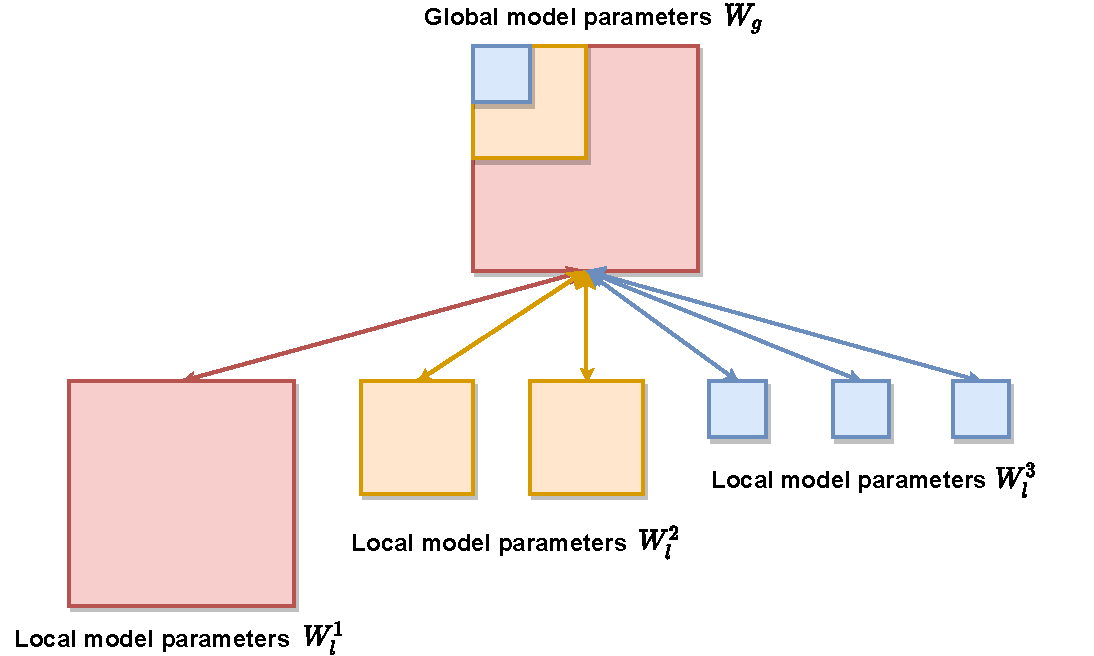
\includegraphics[width=\linewidth]{figs/heterofl_concept.pdf}
  \caption{HeteroFL における幅スケーリングとパラメータ配布
    （文献\cite{HeteroFL} の Figure 1 より引用）．
    グローバルモデル $W_g$（上段）のパラメータを，
    計算複雑度に応じた 3 段階（赤: 大，橙: 中，青: 小）のサブモデルとして
    6 台の端末に配布する．
    小さいモデルのパラメータはすべての端末が保持し，
    大きいモデルのみが持つパラメータは対応する端末のみが保持する．}
  \label{fig:heterofl_concept}
\end{figure}

一方，HeteroFL はすべての端末が同じアーキテクチャ（例: ResNet）を使うことを前提としており，
CNN の畳み込みカーネルと ViT のアテンション重みは構造が根本的に異なるため，
両者を混在させた学習には対応していない．

\subsection{アーキテクチャ異種性への対応}

異なるアーキテクチャ間での知識共有を実現するアプローチとして，
知識蒸留（Knowledge Distillation; KD）を活用した手法が複数提案されている．

Lin ら\cite{FedDF}は，各端末のモデルをアンサンブルし，
その出力を蒸留することで共有データセット上でサーバモデルを訓練する FedDF を提案した．
ただし FedDF はサーバ側での蒸留に公開データセットを必要とするという制約がある．

FedGen\cite{FedGen}はこの制約を克服し，
サーバ側に Generator を配置することで，外部データなしに知識蒸留を実現する．
FedGen の Generator が生成するのは生の画像ではなく，
\textbf{クラスラベルを条件とした仮想潜在ベクトル}——モデルの中間層特徴に相当する低次元ベクトル——である．
各端末はこの仮想潜在ベクトルを自身の分類器（最終層）に直接入力し，
その出力確率分布がサーバ側の複数端末モデルの予測の平均（アンサンブル出力）に近づくよう学習する．
仮想潜在ベクトルが「分類器への入力」として機能するため，
バックボーンのアーキテクチャが端末によって異なっていても同一の教師信号を使えるという点が，
アーキテクチャ非依存な知識共有を可能にする仕組みである（図~\ref{fig:fedgen_overview}）．

\begin{figure}[htb]
  \centering
  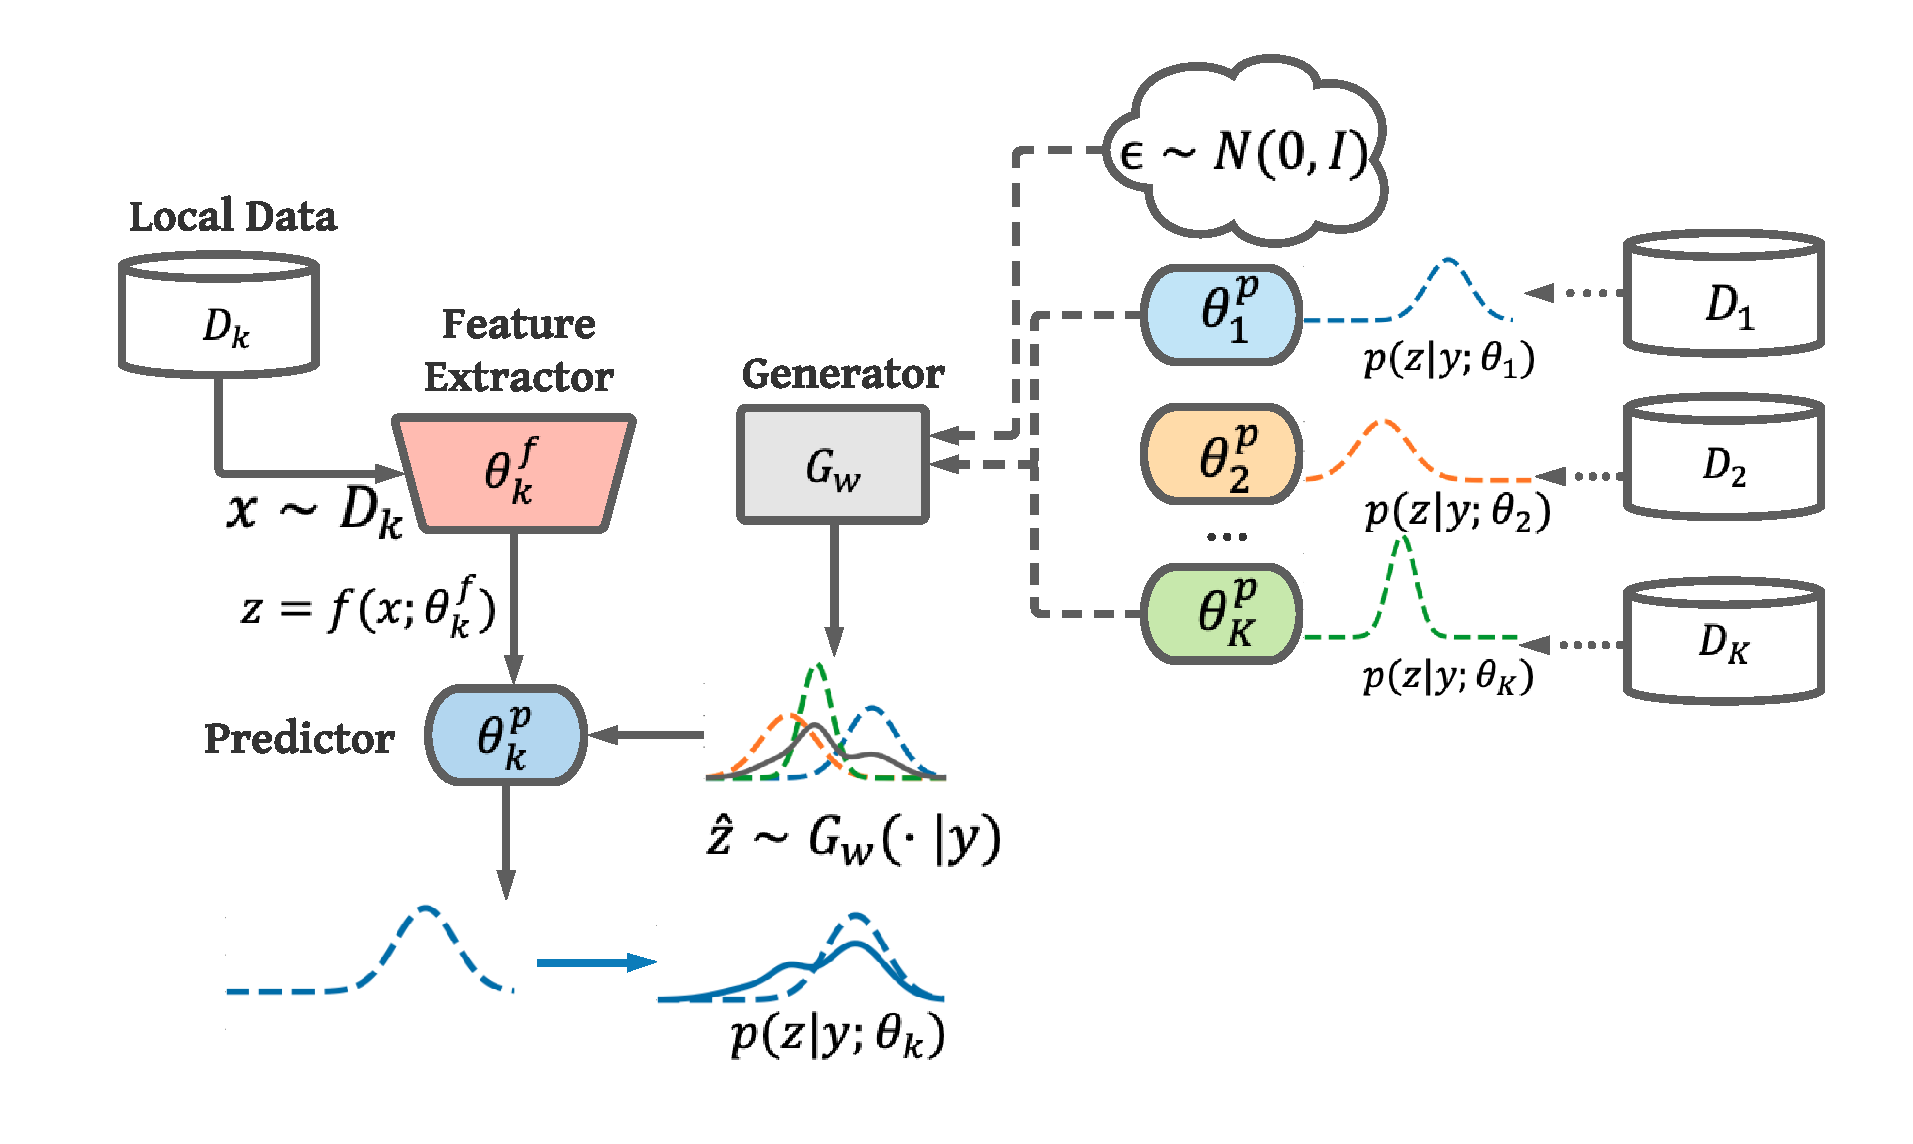
\includegraphics[width=\linewidth]{figs/fedgen_overview.pdf}
  \caption{FedGen のシステム概要
    （文献\cite{FedGen} の Figure 1 より引用）．
    サーバ上の Generator $G_\mathbf{w}$ が，
    各端末の Predictor（$\theta_k^p$）の予測分布に整合する
    仮想潜在ベクトル $\hat{z} \sim G_\mathbf{w}(\cdot|y)$ を生成する（右上）．
    各端末はこの仮想潜在ベクトルを自身の Predictor に入力し（左下），
    アンサンブル出力に近づくよう学習することで，
    外部データなしに端末間の知識蒸留を実現する．}
  \label{fig:fedgen_overview}
\end{figure}

しかし FedGen は全端末が同一サイズのモデルを持つことを前提としており，
端末間でモデルの幅（チャネル数）が異なる計算異種性への対応は考慮されていない．

\subsection{モデル集約の高度化}

Wang ら\cite{FedMA}はニューロンのパーミュテーション不変性を利用して
モデルをマッチングしながら集約する FedMA を提案した．
FedMA は同一アーキテクチャのモデル間での集約精度を向上させるが，
異なるアーキテクチャ間での適用は困難である．

\subsection{既存手法の整理}

表~\ref{tab:related}に，AFAD と関連手法の比較を示す．
計算異種性とアーキテクチャ異種性の両方を同時に扱う手法は，
AFAD 以前には存在しなかった．

\begin{table}[hbt]
  \centering
  \caption{連合学習関連手法の比較}
  \label{tab:related}
  \begin{tabular}{lp{1.2cm}p{1.5cm}p{1.2cm}}
    \toprule
    手法 & 計算\newline 異種性 & アーキテクチャ\newline 異種性 & 外部データ\newline 不要 \\
    \midrule
    FedAvg\cite{McMahanFedAvg}  & \texttimes & \texttimes & \checkmark \\
    FedProx\cite{FedProx}       & \texttimes & \texttimes & \checkmark \\
    HeteroFL\cite{HeteroFL}     & \checkmark & \texttimes & \checkmark \\
    FedDF\cite{FedDF}           & \texttimes & \checkmark & \texttimes \\
    FedGen\cite{FedGen}         & \texttimes & \checkmark & \checkmark \\
    \textbf{AFAD（提案手法）}       & \checkmark & \checkmark & \checkmark \\
    \bottomrule
  \end{tabular}
\end{table}

%----------------------------------------------------------------------
